\documentclass[10pt]{article}
\usepackage{graphicx}
\usepackage[margin=1.5cm]{geometry}
\usepackage{amsmath}
\def\brcurs{{\mbox{$\resizebox{.16in}{.08in}{
\includegraphics{BoldR}}$}}}
\def\rcurs{{\mbox{$\resizebox{.16in}{.08in}{
\includegraphics{ScriptR}}$}}}

\begin{document}
\twocolumn

\title{Tuesday Warm-up: Electric Fields in Matter}
\author{Prof. Jordan C. Hanson}

\maketitle

\section{Memory Bank}

\small

\begin{itemize}
\item \textbf{Gradient} in spherical coordinates:
\begin{equation}
\nabla V = \frac{\partial V}{\partial r}\hat{\mathbf{r}}+\frac{1}{r}\frac{\partial V}{\partial \theta}\hat{\boldsymbol{\theta}} + \frac{1}{r\sin\theta}\frac{\partial V}{\partial \phi}\hat{\boldsymbol{\phi}}
\end{equation}
\item \textbf{Product Rule 5} for use in integration by parts:
\begin{equation}
\nabla \cdot (f\mathbf{A}) = f (\nabla \cdot \mathbf{A}) + \mathbf{A} \cdot (\nabla f)
\end{equation}
\item \textbf{Potential of a dipole} with dipole moment \textbf{p}:
\begin{equation}
V(\mathbf{r}) = \frac{1}{4\pi\epsilon_0}\frac{\mathbf{p} \cdot \brcurs}{\rcurs^2}
\end{equation}
\item \textbf{Polarizability} $\alpha$ of atom or molecule with induced dipole moment $\mathbf{p}$, in external field $\mathbf{E}$:
\begin{equation}
\mathbf{p} = \alpha \mathbf{E}
\end{equation}
\item \textbf{Torque} on a dipole with dipole moment $\mathbf{p}$ in an external field $\mathbf{E}$:
\begin{equation}
\mathbf{N} = \mathbf{p} \times \mathbf{E}
\end{equation}
\item Given the \textbf{polarization per unit volume, P}:
\begin{itemize}
\item Bound volume charge: $\rho_{\rm b} = -\nabla \cdot \mathbf{P}$
\item Bound surface charge: $\sigma_{\rm b} = \mathbf{P} \cdot \hat{\mathbf{n}}$
\end{itemize}
\end{itemize}

\begin{figure}
\centering
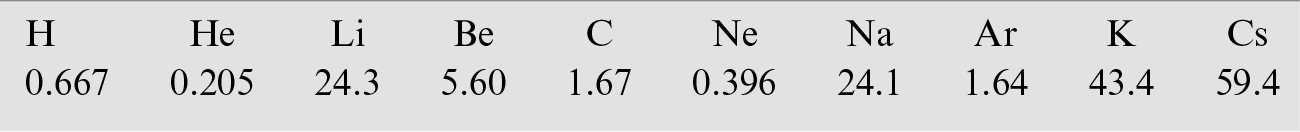
\includegraphics[width=0.49\textwidth]{figures/tab1.jpg}
\caption{\label{fig:1} Atomic polarizabilities, in units of $\alpha/(4\pi\epsilon_0)\times 10^{-30}$, for various atomic elements.}
\end{figure}

\begin{figure}
\centering
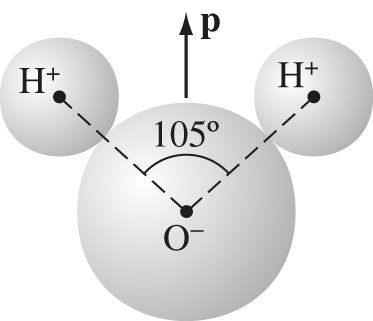
\includegraphics[width=0.15\textwidth]{figures/4_4.jpg} \hspace{1cm}
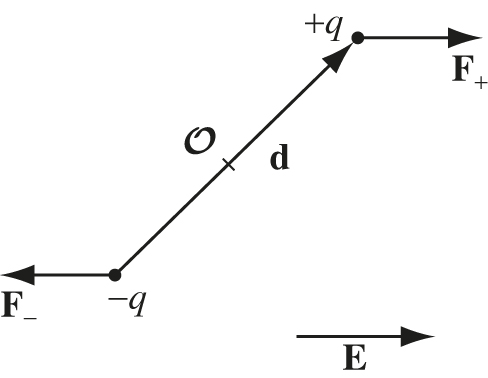
\includegraphics[width=0.2\textwidth]{figures/4_5.jpg}
\caption{\label{fig:2} (Left) Water is an example of a \textit{polar molecule.} (Right) Molecules with dipole moments experience a torque in an external field.}
\end{figure}

\section{Vector Calculus Technique}

\begin{enumerate}
\item Let $f = 1/r$, and $\mathbf{A} = A\hat{\mathbf{r}}$. (a) Use product rule 5 (Memory Bank) to compute $\nabla \cdot (f\mathbf{A})$. (b) Use product rule 5 (Memory Bank) to rearrange the following volume integral over a sphere of radius $R$:
\begin{equation}
\int \mathbf{A} \cdot (\nabla f) d\tau'
\end{equation}
(c) Use the divergence theorem to switch the volume integral into a surface integral. (d) Complete the integral. \\ \vspace{2.5cm}
\end{enumerate}

\section{Polarizable Atoms and Molecules}

\begin{enumerate}
\item Suppose an atom consists of a point charge $+q$ and a uniformly charged sphere with radius $a$ and total charge $-q$, both centered at the origin. (a) Use Gauss' law to calculate the field due to the negatively charged cloud a distance $d$ from the origin. (b) Suppose this field strength is equal and opposite to the field pulling on $+q$.  Calculate the ratio $\alpha$ between $p = qd$ and the field strength. (c) Show that $\alpha/(4\pi\epsilon_0)$ has units of volume.\footnote{Note: the units of $\epsilon_0$ are Farads per meter.}\\ \vspace{2.5cm}
\item Suppose a dipole consisting of two equal and opposite charges is placed in an external field.  Prove the torque on the dipole is $\mathbf{N} = \mathbf{p} \times \mathbf{E}$. \\ \vspace{2cm}
\item Suppose a sphere has a uniform polarization $\mathbf{P}$.  What are the (a) $\sigma_{\rm b}$ and (b) $\rho_{\rm b}$? (c) Which Legendre polynomial does the charge distribution resemble?
\end{enumerate}

\end{document}
